\section{RunDroid系统的设计与实现 }
\label{ch3}

\subsection{系统功能介绍}
本文以帮助研究人员和开发人员了解Android应用程序的执行过程作为基本出发点,通过设计与实现Android动态函数调用图构建系统RunDroid,生成Android应用程序运行时对应的动态函数调用图,从方法调用关系、方法间的触发关系以及方法执行的相关对象信息等多个方面较为全面地展现Android应用的执行过程,为应用程序分析提供更为多样、准确的信息。另外,系统具备一定的可拓展性,可以方便相关人员根据自身的业务需求对系统进行扩展,完成相应的需求。

\subsection{概念定义}
\eat{
\define{
    图:图是是对节点和边的描述,通常使用二元组$G(V,E)$表示。对于图中的节点$v$, $v \in V$;对于图中的边 $e$, $e \in E$。
}
\define{
    有向图:按照图中的边是否区分方向,我们可以将图分为有向图和无向图。
}
}


\define{
    调用(Invoke):对于程序$P$的两个方法$m_1$和$m_2$,如果在方法$m_1$中调用了方法$m_2$,则记作$m_1 \to m_2$,称为方法$m_1$调用方法$m_2$。
}
\begin{equation}
m_0 \to m_1 \to \dots m_{n - 1} \to m_n  \label{equ:extend_invoke}
\end{equation}

    在此基础上,对于方法$m_0$和方法$m_n$,若存在方法$m_i$($i=1,\dots,n-1,n>1$),使得~\ref{equ:extend_invoke}成立,,则记作$m_0 \stackrel{\ast}{\to} m_n$,称为方法$m_0$扩展调用方法$m_n$。


    补充的,对于方法$m_1$和方法$m_2$,若$m_1 \to m_2$,也可以记为$m_1  \stackrel{\ast}{\to}  m_2$。

\define{
    函数调用图(CallGraph,CG):函数调用图$CG = ( V , E)$是一个有向图(DAG), 图中的点$ v \in V $表示一个\textbf{方法实体} $m$;
    如果方法$m_1$调用方法$m_2$(即$m_1 \to m_2$),则有向边 $e = (m_1 ,m_2)$属于集合 $E$。 
}

\define{
    动态函数调用图(Dynamic CallGraph,DCG):动态函数调用图是在调用图的基础上演化而来,是对程序运行时行为的描述。
    同样的,动态函数调用图也是一个有向图($DCG = ( V , E)$)。 图中的点$ v \in V $表示一个\textbf{方法执行} $m$;
    如果方法$m_1$调用方法$m_2$(即$m_1 \to m_2$),则有向边 $e = (m_1 ,m_2)$属于集合 $E$。 
}

\textbf{注意:}函数调用图和动态函数调用图是分别从静态分析角度和动态分析角度对程序运行过程的描述。
前者分析的整体是方法实体,是静态分析的结果,每次产生的结果是一样的;
后台则为方法执行,是对动态行为的描述,每次产生的结果和具体的执行过程相关,不一定是一样的。

例如,方法A调用了方法B,函数调用图$CG$如~\ref{equ:cg_sample}所示。
但若,在实际执行过程中,方法A被调用了两次,这对应的动态函数调用图$DCG$如~\ref{equ:dcg_sample}所示。
可以看出,$DCG$中,$method_a$ 和 $method_b$ 各有两个,分别对应的两次\textbf{函数执行}。
\begin{equation}
CG = ({method_a,method_b},{(method_a \to method_b )} ) \label{equ:cg_sample}
\end{equation}

\begin{equation}
\begin{aligned}
DCG = &(V,G) ,\\ 
V = & \{method_{a_{(1)}},method_{b_{(1)}},method_{a_{(2)}},method_{b_{(2)}}\}, \\ 
G = & \{  
    (  method_{a_{(1)}} \to method_{b_{(1)}}) ,( method_{a_{(2)}} \to method_{b_{(2)}})
 \} 
\end{aligned}
\label{equ:dcg_sample} 
\end{equation}


\define{
    方法对象(Method Object,MO):
和方法执行相关的对象称为方法对象,可以体现对象和执行方法的相互关系。
具体的,在一次具体的方法执行过程中,
如果对象$p$是这个方法$m$的参数,记为$p \stackrel{parameter}{\longrightarrow} m$;
如果对象$r$是这个方法$m$的返回值,记为$r \stackrel{return}{\longrightarrow} m$;
若方法$m$是非静态方法,则方法执行时我们可以获取到关联到的this指针对象$i$,记为$i \stackrel{instance}{\longrightarrow} m$;
}


\define{
    触发关系(Trigger):
    如果对于动态函数调用图$DCG$中两个方法(不妨记为$m_a$和$m_b$,$m_a \in DCG$,$m_b \in DCG $),若方法$m_a$和方法$m_b$之间同时需要满足以下三个条件,
    则两个方法存在触发关系,记为$m_a \hookrightarrow m_b$,称为$m_a$触发了$m_b$:
    
\begin{enumerate}
  \item 方法$m_a$的执行时间总是在方法$m_b$的执行时间之前;
  \item $m_a \stackrel{\ast}{\to} m_b $不成立;
  \item $m_a$、$m_b$之间存在着一定的因果关系,包括但不限于生命周期事件,UI交互事件或多线程通信等。
\end{enumerate}
}

\define{
    拓展动态函数调用图(Extended Dynamic CallGraph,EDCG):在动态函数调用图(DCG)的基础上,添加了方法对象和函数间的触发关系。
    拓展动态函数调用图中的节点包括方法执行节点和方法对象节点。图中的边包括描述方法间关系的边和描述方法和对象间的边:
    前者的方法间关系包括调用关系和触发关系;而后者的关系包括和方法对象相关的三个关系。
    具体定义如~\ref{equ:def_edcg}所示:

\begin{equation}
\begin{aligned}
EDCG = & (V_{EDCG},E_{EDCG}) ,\\ 
DCG = & (V_{DCG},E_{DCG}) ,\\ 
V_{EDCG} = & V_{method} \bigcup V_{object} ,\\
V_{method} = & V_{DCG}, \\ 
G_{EDCG} = & G_{method} \bigcup G_{object} , \\
G_{method} = & E_{DCG} \bigcup \{ (m_1 , m_2) m_1 \hookrightarrow m_2 \}
\end{aligned}
\label{equ:def_edcg} 
\end{equation}
    
}

\subsection{ 设计思路介绍}
以下面一段代码里为例,我们将简要介绍一下RunDroid还原Android应用程序动态函数调用图的基本思路:
~\ref{fig:code_sample}-左为一段面向过程编程的示例代码,当main函数执行时,会一次调用A、B两个函数,而B函数有调用了C、D两个函数,
对应动态函数调用图如~\ref{fig:code_sample}-右所示。
 
 
 \begin{figure*}
	\centering
	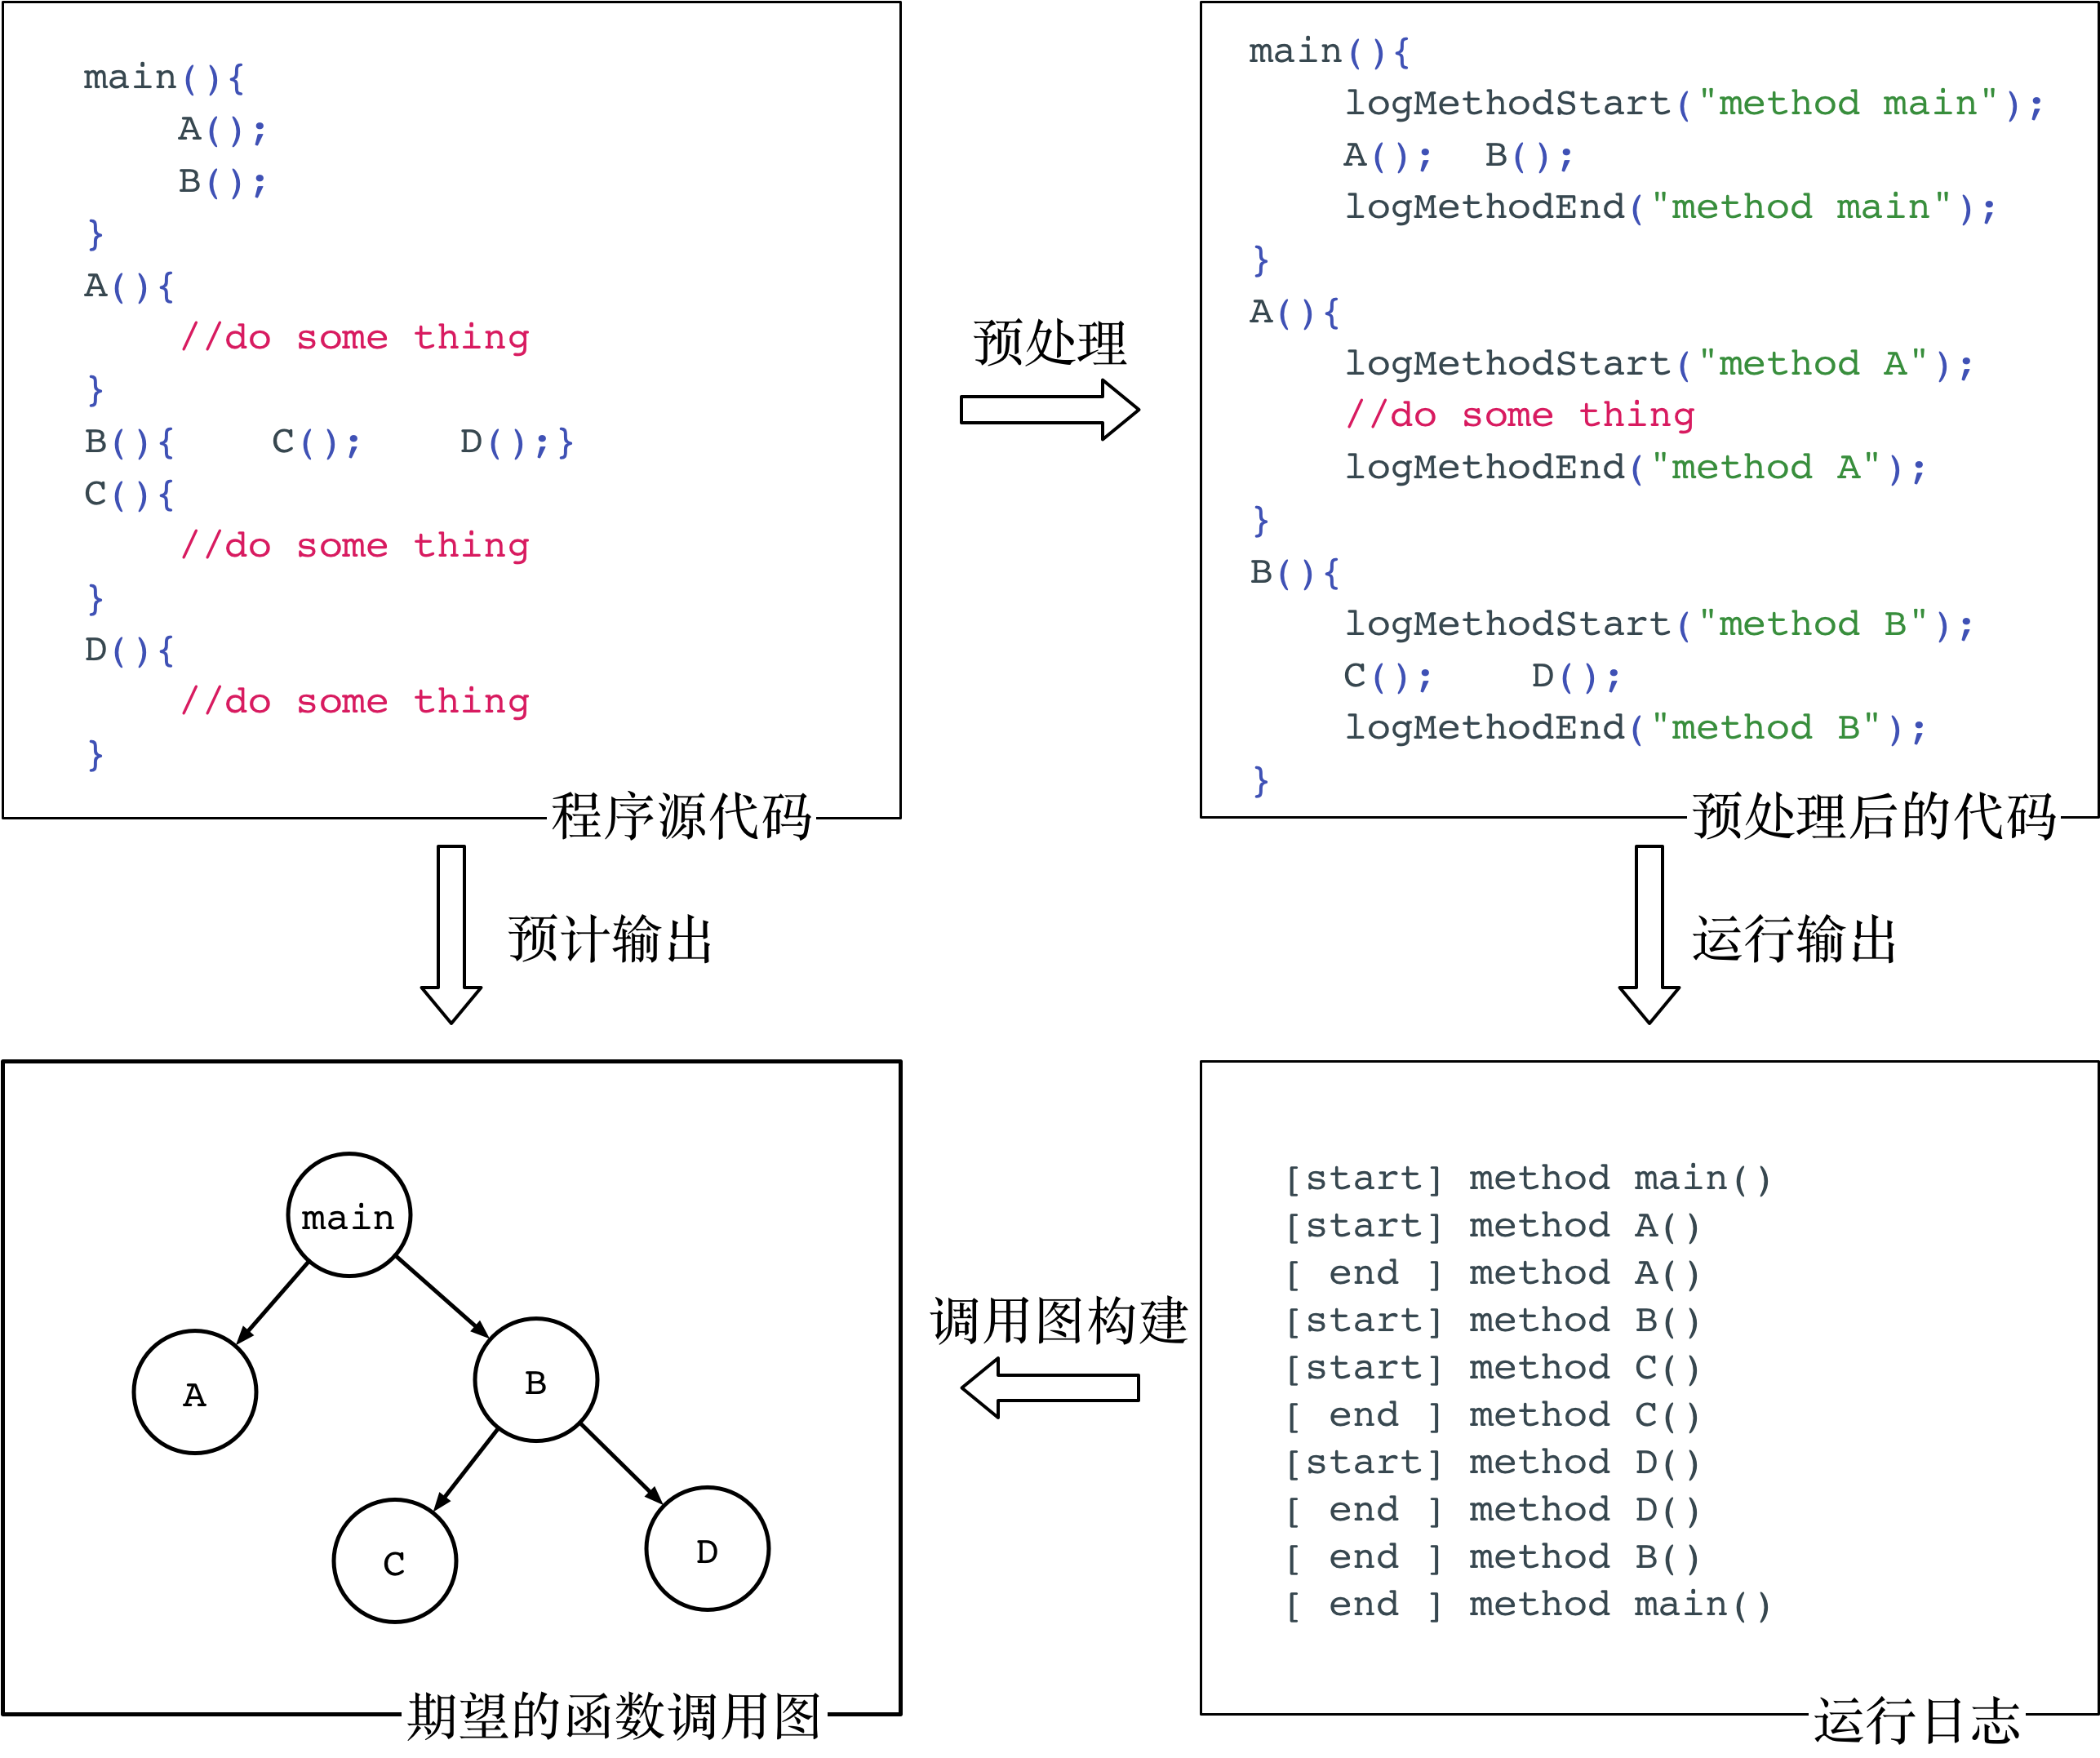
\includegraphics[width=\textwidth]{./Figures/code-sample.png}
	\caption{ 面向过程编程语言的函数调用的示例}
	\label{fig:code_sample}
\end{figure*}


从函数调用图的构建过程可以看出,程序的执行过程就是对函数调用图自上而下的深度优先遍历过程。由此可见,若要还原出图 6-右中的函数调用图,本文采用的基本思路是以日志方式输出对右图中的函数调用图的深度优先遍历序列,并基于得到的遍历序列还原出函数调用图。
由于Android是由面向对象编程语言Java开发的系统,系统还需要考虑面向对象编程的特性——多态性(即同一个行为在不同的对象下的表现可以不同)。为此,RunDroid还会在函数调用图将函数执行和对应的对象进行关联,更好地体现面向对象编程的函数调用关系。基于上述的函数调用关系的信息,RunDroid根据函数调用之间的关系进一步挖掘,进一步挖掘Android系统中的特性(例如组件Activity的生命周期、多线程的交互方式)。

\subsection{技术路线(偏工程性)}
本技术路线拟利用语法分析工具,对Android应用程序进行了应用源代码层面的执行日志插桩工作,利用非侵入式系统行为修改插件获取系统层面的函数执行信息。结合以上日志信息,方案对日志进行初步处理,在图数据库上构建原始的Android应用程序的动态函数调用图。通过阅读分析Android系统中多线程相关的源代码,制定具体的多线程分析插件,进而在函数调用图中标识出多线程相关的方法间触发关系,全面地展现Android应用的执行过程。
 
 
\begin{figure*}
\centering
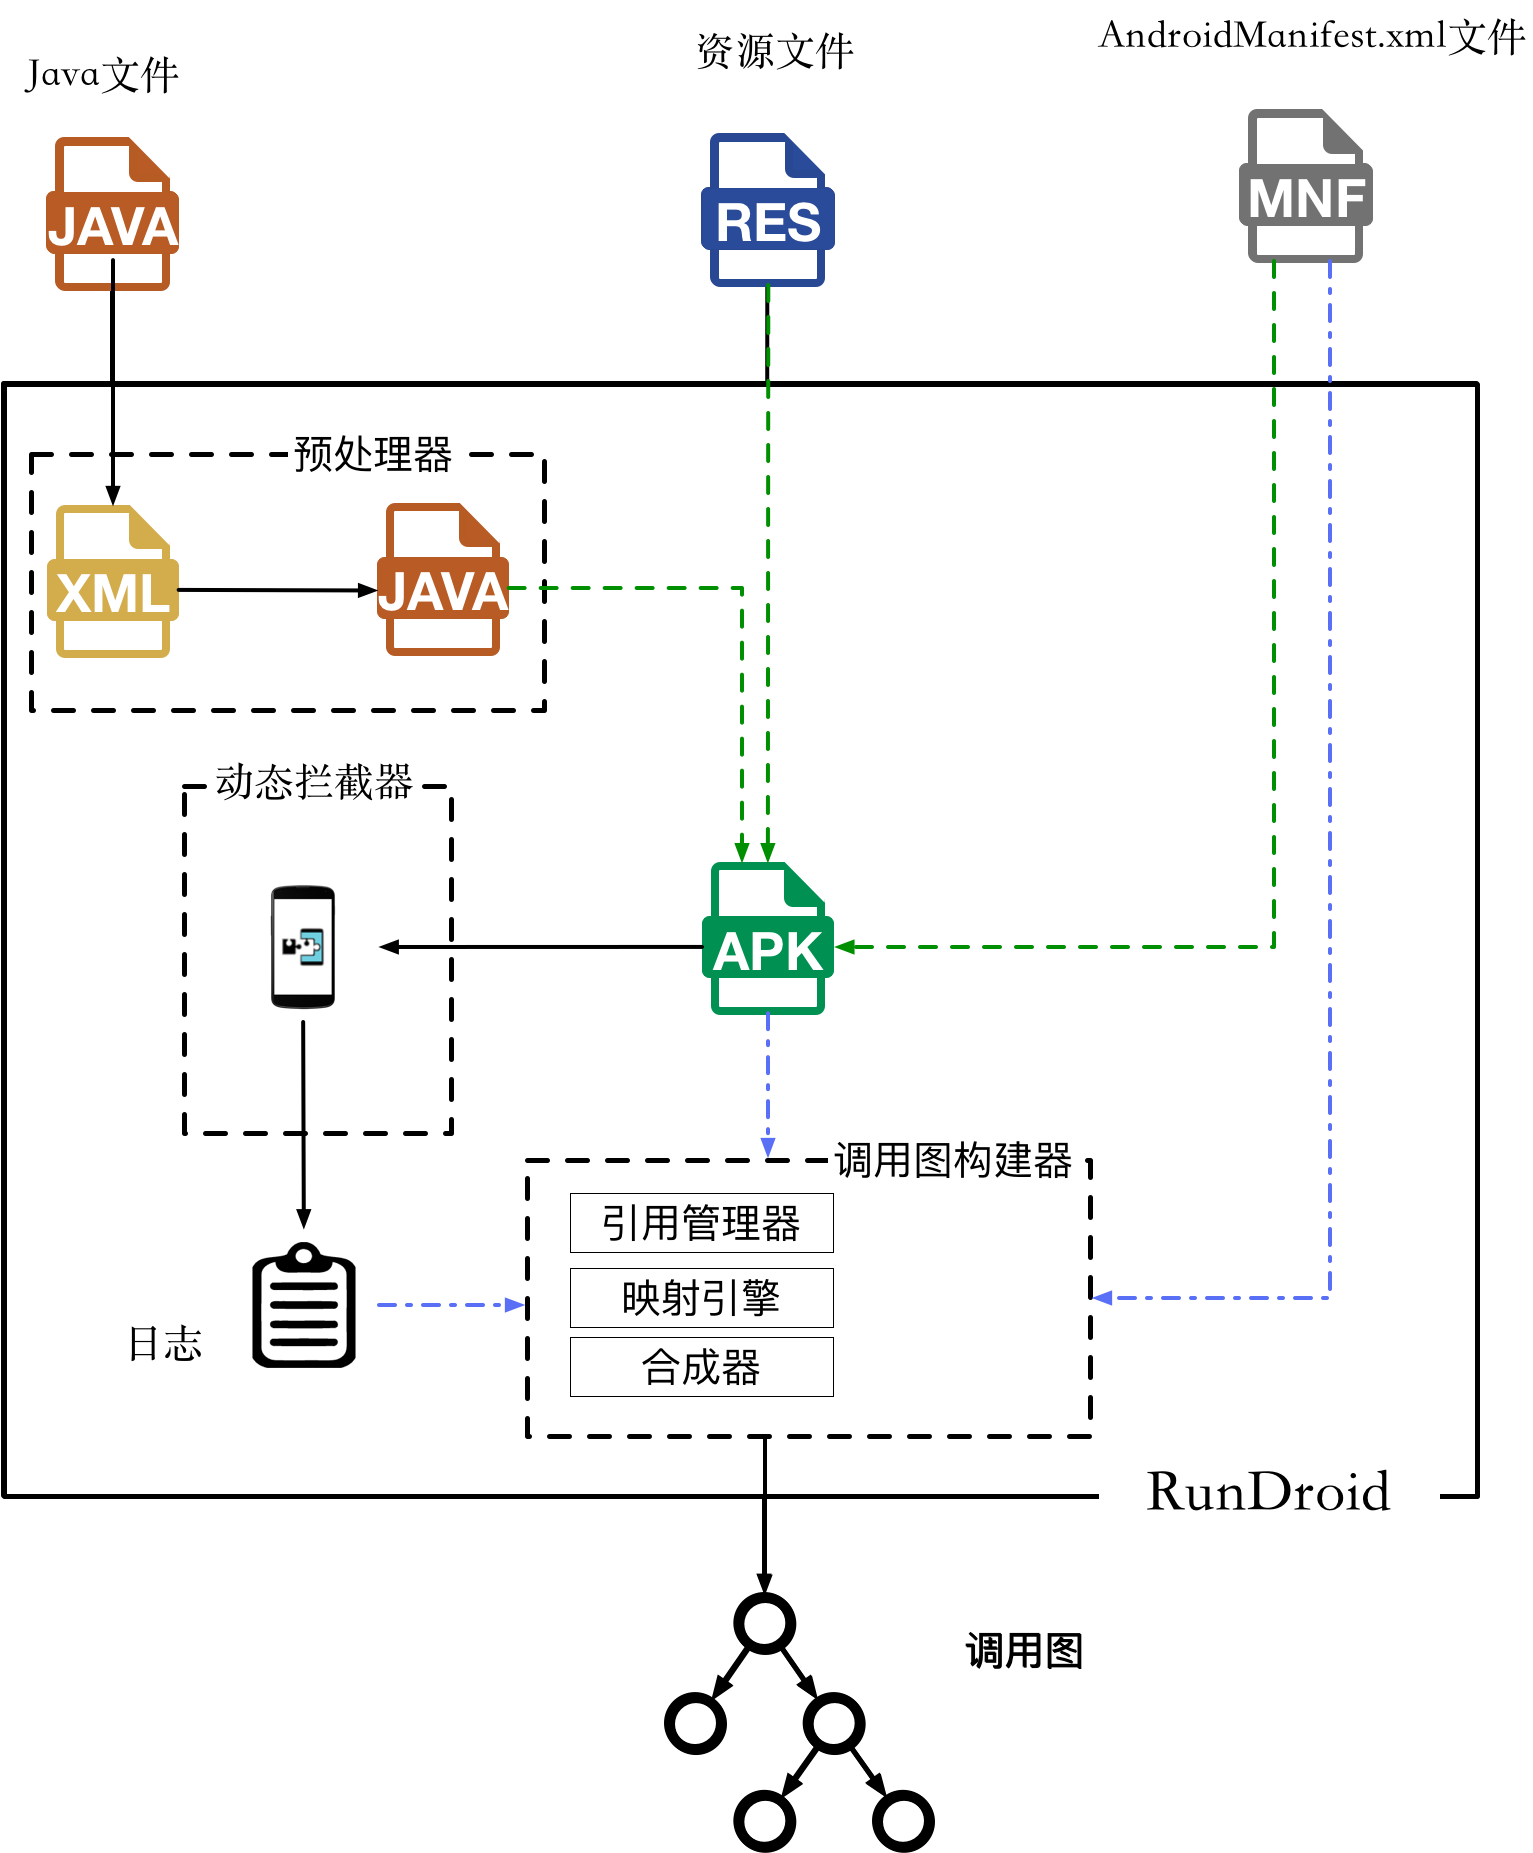
\includegraphics[width=\textwidth]{./Figures/rundroid-overview.png}
\caption{ RunDroid基本架构图}
\label{fig:rundroid_overview}
\end{figure*}


\subsection{相关技术介绍}

\subsubsection{	srcML介绍}

\subsubsection{Xposed框架介绍}
Xposed是由rovo89主导开发的第三方框架。基于Xposed开发的第三方插件,可以在不修改系统和应用程序源代码的情况下,改变他们的运行行为。Xposed框架可以运行在不同版本的Android系统上,开发过程十分便利,而且易于撤销。Xposed的实现原理具体如下:由于Android系统的所有的应用程序进程都是由Zygote进程孵化而来,Xposed通过替换/system/bin/app\_process程序,使得系统在启动过程中加载Xposed的相关文件,将所有的目标方法指向Native方法xposedCallHandler,维护目标方法和对应的钩子方法(Hook Function)的映射关系,从而实现对Zygote进程及Dalvik虚拟机的劫持;当程序执行到目标方法时,xposedCallHandler会完成目标方法的原有代码和对应钩子方法的调度,达到对目标方法劫持的目的。使用Xposed,可以帮助我们实现类似面向切面编程(Aspect-Oriented Programming, AOP)的功能,完成系统层面的方法执行情况的记录。
\subsubsection{	Neo4j介绍}
Neo4j是基于Java语言开发的图数据库。与传统的基于关系模型的存储结构不同,Neo4j的存储模型是基于图论开发的,遵循属性图数据模型。Neo4j的数据主要分为节点(Node)和关系(Relationship)两大类,另外,Neo4j还可以在关系和节点上添加key-value形式的属性,为节点指定一个或者多个标签,为关系指定类型等等。Neo4j以Lucence作为索引支撑,支持完整的 ACID(原子性,一致性,隔离性和持久性)事务规则,提供了基于Cypher脚本、Native Java API和REST Http API等多种方式帮助开发人员进行数据开发工作。同时,Neo4j还提供了友好的浏览器界面,具有十分友好的交互体验。由于基于属性图数据模型,Neo4j通常适用于和图关系有着密切关系的应用场景:例如社交网络分析,公共交通网络研究以及地图网络拓扑等场景。在RunDroid,Neo4j主要承担着函数调用图的数据存储和查询的主要职责。

\subsection{模块实现介绍}


\subsubsection{源代码预处理组件(Preprocessor)}

\subsubsection{	运行时日志记录器(Runtime Logger)}

\subsubsection{调用图构建器(Call-graph Builder)}

\subsection{构建过程介绍}


\subsubsection{如何构建函数调用图}

算法:
输入:
输出:
过程:
写一段
写一段
写一段
写一段
写一段
写一段
写一段

\subsubsection{如何构建Activity的生命周期}

\subsubsection{	如何构建多线程触发关系}

\subsection{本章小结}
